\documentclass[11pt,preprint, authoryear]{article}

\pagestyle{plain}

\usepackage{lmodern}

% spacing passed through from .Rmd doc
\usepackage{setspace}
\setstretch{1.5}

% Wrap around which gives all figures included the [H] command, or places it "here". This can be tedious to code in Rmarkdown.
\usepackage{float}
\let\origfigure\figure
\let\endorigfigure\endfigure
\renewenvironment{figure}[1][2] {
    \expandafter\origfigure\expandafter[H]
} {
    \endorigfigure
}

\let\origtable\table
\let\endorigtable\endtable
\renewenvironment{table}[1][2] {
    \expandafter\origtable\expandafter[H]
} {
    \endorigtable
}

\usepackage{ifxetex,ifluatex}
\usepackage{fixltx2e} % provides \textsubscript
\ifnum 0\ifxetex 1\fi\ifluatex 1\fi=0 % if pdftex
  \usepackage[T1]{fontenc}
  \usepackage[utf8]{inputenc}
\else % if luatex or xelatex
  \ifxetex
    \usepackage{mathspec}
    \usepackage{xltxtra,xunicode}
  \else
    \usepackage{fontspec}
  \fi
  \defaultfontfeatures{Mapping=tex-text,Scale=MatchLowercase}
  \newcommand{\euro}{€}
\fi

\usepackage{amssymb, amsmath, amsthm, amsfonts}

\DeclareMathSizes{24}{26}{22}{22}

\usepackage[round]{natbib}
\bibliographystyle{natbib}
\def\bibsection{\section*{References}} %%% Make "References" appear before bibliography

% package for nice tables
\usepackage{longtable}

% package for ruling lines in tables
\usepackage{booktabs}

% set margins
\usepackage[left=3.5cm, right=2cm, top=30mm ,bottom=2cm, includefoot]{geometry}
\usepackage{fancyhdr}
\usepackage[bottom, hang, flushmargin]{footmisc}
\usepackage{graphicx}
\numberwithin{equation}{section}
%\numberwithin{figure}{section} % commented out because it messes up figure numbering
%\numberwithin{table}{section} % commented out because it messes up table numbering
\setlength{\parindent}{0cm}
\setlength{\parskip}{1.3ex plus 0.5ex minus 0.3ex}
\usepackage{textcomp}
\renewcommand{\headrulewidth}{0pt}

\usepackage{array}
\newcolumntype{x}[1]{>{\centering\arraybackslash\hspace{0pt}}p{#1}}

\usepackage{hyperref}
\hypersetup{breaklinks=true,
            bookmarks=true,
            colorlinks=true,
            citecolor=blue,
            urlcolor=blue,
            linkcolor=blue,
            pdfborder={0 0 0}}
						
\urlstyle{same}  % don't use monospace font for urls
\setlength{\parindent}{0pt}
\setlength{\parskip}{6pt plus 2pt minus 1pt}
\setlength{\emergencystretch}{3em}  % prevent overfull lines
\setcounter{secnumdepth}{5}

% Use protect on footnotes to avoid problems with footnotes in titles
\let\rmarkdownfootnote\footnote%
\def\footnote{\protect\rmarkdownfootnote}
\IfFileExists{upquote.sty}{\usepackage{upquote}}{}

% pass through extra packages specified by user
\usepackage{bm}

%%%%%%%%%%%%%%%%%%%%%%%%%%%%%%%%%%%%%%%%%%%
%%%%%%%%%%%%%%%%%% EDIT TITLE %%%%%%%%%%%%%%%%%%
%%%%%%%%%%%%%%%%%%%%%%%%%%%%%%%%%%%%%%%%%%%

% change title format to be more compact
\usepackage{titling}

% create subtitle command for use in maketitle
\newcommand{\subtitle}[1]{
  \postauthor{
    \begin{center}\large#1\end{center}
    }
}

\setlength{\droptitle}{-1em}
\pretitle{\vspace{\droptitle}\centering\Huge}
\posttitle{\par\vskip 5.5em}

\title{
{\scshape\Large Department of Statistics 2019}\\
{\vskip 2.5em \scshape Predicting Community Engagement with Questions Across Online
Question-Answer Fora}\\
%{\includegraphics{lse.png}} % if you want to include LSE logo
}

\preauthor{\centering\LARGE}
\postauthor{\par\vskip 4em}

\author{Candidate Number: 10140}
\subtitle{\vspace{4em} Submitted for the Master of Science, London School of Economics,
University of London} % comment this out and you get *Missing \begin{document}*

\predate{\centering\Large}
\postdate{\par}

\date{\scshape August 2019}

\usepackage{color}
\usepackage[usenames,dvipsnames,svgnames,table]{xcolor}
\usepackage{hyperref}
\hypersetup{
     colorlinks = true,
     citecolor = gray
}

\usepackage{tocloft}

\renewcommand{\cftsubsecfont}{\normalfont\hypersetup{linkcolor=black}}
\renewcommand{\cftsubsecafterpnum}{\hypersetup{linkcolor=black}}

%%%%%%%%%%%%%%%%%%%%%%%%%%%%%%%%%%%%%%%%%%%
%%%%%%%%%%%%%%%% BEGIN DOCUMENT %%%%%%%%%%%%%%%%
%%%%%%%%%%%%%%%%%%%%%%%%%%%%%%%%%%%%%%%%%%%

\begin{document}

% Header and Footers
\pagestyle{fancy}
\chead{}
\rhead{}
\lfoot{}
\rfoot{} 
\lhead{}
%\rfoot{\footnotesize Page \thepage\ } % "e.g. Page 2"
\cfoot{\footnotesize \thepage\\}

% i, ii, iii etc. page numbering
\pagenumbering{roman}

\maketitle

\thispagestyle{empty}

\clearpage

\setcounter{page}{1}

% table of contents, list of figures and tables
\renewcommand{\contentsname}{Table of Contents}
\hypersetup{linkcolor=black}
\tableofcontents
\newpage
\hypersetup{linkcolor=black}
\listoffigures
\newpage
\hypersetup{linkcolor=black}
\listoftables
\hypersetup{linkcolor=black}
\newpage

\section*{Summary}

Formulating constructive questions and receiving answers to these
questions is not only a key part of how we learn, but to scientific
progress and development. The evolution of the world wide web and the
technologies it has provided us has given us an unprecendented ability
to engage with and learn from the world, and while substantial attention
has been dedicated to finding correct answers (just ask Google),
comparitively less has been devoted to how we can improve the
constructiveness of our questions. One online setting where relevant and
well-researched questions is of particular importance is online
question-answer (Q\&A) communities such as Yahoo! Answers, Quora and the
StackExchange family of websites. These knowledge-sharing platforms
often suffer from a problem of scarce professional resources compared to
an abundance of questions, and it is precisely this issue of information
overload that this research aims to address. By successfully predicting
the extent of community engagement with questions using only the textual
content available when a user submits a new question, questioners can be
informed and nudged to improve the ``signal'' of their questions before
adding demand to these communities, thereby improving the functioning
and efficiency of these platforms substantially. I build on work
addressing questions in Q\&A communities and construct models to predict
on the community-granted score of questions for a range of diverse
StackExchange Q\&A communities. My results for topic modelling features
show that community engagement \textbf{can be predicted}, however from
the variation of performance of models across fora it appears that
communities \textbf{engage heterogenously} with questions.

\clearpage

% 1, 2, 3 etc. page numbering
\pagenumbering{arabic}

\newpage

\section{\texorpdfstring{Introduction
\label{Intro}}{Introduction }}\label{introduction}

Modern interpersonal communication technologies made possible by the
internet have afforded us an exceptional level of connection and
engagement with the world. Billions of individuals now interact online
every split second, not only with people that they know, but with
strangers millions of miles away. An extremely popular manner in which
internet users have chosen to engage online is by knowledge sharing
through specific question-and-answer (Q\&A) websites such as Yahoo!
Answers, Quora, the StackExchange family and forums of Massive Online
Open Courses (MOOCs). These websites serve as platforms where users seek
answers to and discussions on \textbf{complex and technical} questions
that modern search engines are evidently yet unable to fully address.

It goes without saying that producing legible, relevant and
well-researched questions in online Q\&A fora is particularly valuable,
not least since platforms are particularly prone to ``information
overload'' where cascades of new questions far outweigh the few expert
resources available. This research aims to address this problem by
determining to what extent positive community engagement can be
predicted using only the textual content of questions - i.e.~a
question's \texttt{Title} and \texttt{Body}.

The broad research question can therefore be defined as the following:

\begin{center}
\emph{To what extent can community engagement with questions in online Q\&A communities be accurately captured and predicted?}
\end{center}

While there is a substantial amount of literature that has addressed
Q\&A fora, it has focused on identifying expert users and high quality
answers rather than given attention to questions, despite questions
being the entry point for every interaction in communities. I draw
heavily on and critique prior research done by Ravi \emph{et al.} (2014)
and analyse question content from the
\href{https://stackexchange.com/sites\#}{StackExchange} family of Q\&A
communities. These Q\&A fora have a voting mechanism whereby registered
community-members can signal how much value specific questions add to
the community and it is precisely this metric which I identify as
community engagement and aim to predict on.

This research goal thus takes the form of quantitative prediction task
rather than qualitative, causal or inferential analysis. I leave it to
further research to address the \emph{how} and \emph{why} of community
engagement on online Q\&A communities, rather than just the \emph{what}
that is explored here. I build a \textbf{elastic net, regularised}
regression model to predict the community-assigned \texttt{Score} for
each question, which is the result of aggregating all community up-votes
and down-votes.

This research thus has a concrete application to the real world:
providing these predictions to questioners in real-time can encourage
them to improve the ``signal'' of their questions before they submit new
questions and add demand to the resources of a community. \textbf{In
this way, it is hoped that the functioning and evolution of these online
communities can be improved.} I believe that the fact that this research
aims to predict a community-provided measurement of online engagement,
has a direct real-life application and will be implemented on
\textbf{diverse communities makes it the first of its kind.}

I find that \textbf{\ldots{}\ldots{}\ldots{}. and I conclude that the
LDA topic model is not universally effective as Ravi \emph{et al.}
(2014) claimed.} \textbf{and evaluate using root-mean-square error
(RMSE)}.

Previous work in the field of questions in online Q\&A fora will now be
discussed in more detail. This will be followed by a discussion of the
data, exploration of the variables included in the model, a description
of the model used, and a presentation and discussion of the results.
Finally, some recommendations for areas of further research and
concluding remarks are made.

\newpage

\section{\texorpdfstring{Literature Review
\label{Lit}}{Literature Review }}\label{literature-review}

\subsection{Question-Answer
Communities}\label{question-answer-communities}

Much research has concerned Q\&A communities - i.e.~on answer quality
(Jeon \emph{et al.}, 2006; Shah and Pomerantz, 2010; Tian, Zhang and Li,
2013), on satisfaction of questioners (Liu, Bian and Agichtein, 2008)
and on the behaviour of so-called ``expert'' community members (Riahi
\emph{et al.}, 2012; Sung, Lee and Lee, 2013). Often, the framework for
Q\&A fora has been the optimising the routing of questions to experts
(Li and King, 2010; Li, King and Lyu, 2011; Zhou, Lyu and King, 2012;
Shah \emph{et al.}, 2018), or question routing in accordance with
answerer interest in the form of a recommendation system (Wu, Wang and
Cheng, 2008; Qu \emph{et al.}, 2009; Szpektor, Maarek and Pelleg, 2013).

The research here contrasts with this prior work on Q\&A fora in that I
focus on the questions rather than user or answer characteristics, not
only owing to questions having received substantially less attention
literature-wise, but because the quality of questions can significantly
impact the quality of answers (Agichtein \emph{et al.}, 2008). Evidently
as questions also serve as the initially entry-point for the question
answering process after which all community engagement follows, I
believe this focus on questions is well-placed and will enhance the
development and functioning of communities.

Another difference is that I place the research problem in a framework
discordant of systems-based optimisation of question-answer matching and
instead focus on predicting community engagement using only question
content. Thus this is aimed at the very real application of potentially
nudging users to update and enhance their question content before
encumbering community resources. Owing to the large intuitive overlap
between question quality and community engagement in Q\&A communities,
the body of work on question quality in Q\&A fora is discussed next.

\subsection{Question Quality}\label{question-quality}

High-quality questions assuredly lead to positive community engagement,
however \textbf{the only difference may be the specific aspects of
question content that communities value across communities.} Thus, while
the literature discussed here refer to measuring and predicting
``question quality'', I assert that ``community engagement'' is a more
robust interpretation of what they are measuring and so for the sake of
discussion I will refer to question quality as well.

Recent work has looking at predicting question quality for the large
Q\&A community \href{http://answers.yahoo.com}{Yahoo! Answers}
(Agichtein \emph{et al.}, 2008; Bian \emph{et al.}, 2009; Li \emph{et
al.}, 2012), but while this dataset has metrics for assessing answer
quality in the form of answer ``up-votes'', it lacks a similarly
community-attributed and objective metric for question quality.
Agichtein \emph{et al.} (2008) thus define question quality using
question semantic features (lexical complexity, punctuation, typos
etc.), Bian \emph{et al.} (2009) manually label 250 questions and Li
\emph{et al.} (2012) combine the number of answers, number of tags, time
until the first answer, author judgement and domain expertise to
construct their ground truth.

Fortunately, my datasets are from the StackExchange family of Q\&A fora
which are rich in community engagement variables like question
up-/down-votes and view-counts. Coming directly from the data, these
metrics are objective rather than human-labelled and are also therefore
not limited in terms of samples from the data (we can use the whole
dataset).

The predictive models employed in the question quality literature have
also evolved substantially. Previous work has modelled question quality
based on the reputation of the questioner, question categories and
lexical characteristics of questions (length, misspelling, words per
sentence etc.) (Agichtein \emph{et al.}, 2008; Bian \emph{et al.}, 2009;
Anderson \emph{et al.}, 2012; Li \emph{et al.}, 2012).

A fundamental distinction is that I use only the features available at
the time a question is initially asked which is congruent with the goal
of being able to provide real-time information to questioners before
they submit questions to a community. I also don't use any features
derived from user attributes, since doing otherwise would not work well
for questions asked by new users.

\subsection{\texorpdfstring{Ravi \emph{et al.}
(2014)}{Ravi et al. (2014)}}\label{ravi2014}

A paper that made much headway in the classification and prediction of
what they assume is question quality is Ravi \emph{et al.} (2014), who
use the largest and oldest StackExchange site,
\href{https://stackoverflow.com}{StackOverflow} I mirror much of the
analysis in Ravi \emph{et al.} (2014), however I believe I build on
their analysis significantly and distinctly in a number of ways.

Firstly, as mentioned the literature speaks a lot about ``question
quality'' and Ravi \emph{et al.} (2014) decide to incorporate a
question's \texttt{Score} into their ground truth for question quality,
yet I posit that what these studies are measuring is instead more
accurately characterised as community engagement. My opinion is that
question quality is much more nuanced than prior research has asserted,
i.e.~while most communities will value universal aspects of questions
like legibility, coherence, relevance and prior-research, it is
difficult to accurately define how much of this contributes to a
universal inherent ``quality'' objectively compared to
community-specific traits that communities will naturally value
(i.e.~closed-end questions in the natural sciences, discussion-promoting
for social sciences). Thus while I also incorporate the \texttt{Score}
metric into a response variable, my characterisation of this ground
truth as community engagement is broader and more inclusive.

Another departure from the analysis in Ravi \emph{et al.} (2014) that I
make, is I consider a far more diverse range of communities to compare
how models perform across fora. Ravi \emph{et al.} (2014) specifically
state that ``{[}their{]} methods do not rely on domain-specific
knowledge'' and therefore ``{[}they{]} believe {[}the methods{]} are
applicable to other CQA settings as well'' - this is something I
particularly want to test and believe will be interesting to flesh out.

A last distinction between my analysis and Ravi \emph{et al.} (2014) is
that they treat the research aim as a classification problem, quite
arbitrarily defining a threshold for their response variable to
distinguish between ``good'' and ``bad'' questions. Despite
\textbf{making it a more complex problem}, I opt to predict on a
continuous response since that would provide a better indication to
users of how well it is predicted that a community will react to their
question.

Ravi \emph{et al.} (2014) manage impressive results however: using
textual features and latent topics extracted from question content
(i.e.~question \texttt{Title} and \texttt{Body}), their predictions on
\texttt{Score}/\texttt{ViewCount} yield accuracy levels of 72\% on their
StackOverflow dataset. I will be emulating this part of their research,
and thus a discussion of topic modelling is necessary.

\subsection{\texorpdfstring{Topic Modeling
\label{model_lit}}{Topic Modeling }}\label{topic-modeling}

Bayesian models have recently achieved immense popularity to solve a
diverse range of structured prediction challenges in Natural Language
Processing (NLP) (Chiang \emph{et al.}, 2010). Blei, Ng and Jordan
(2003) presented Latent Dirichlet Allocation (LDA) topic models as
generative Bayesian models for documents to uncover hidden topics as
probability distributions over words. LDA can therefore be useful in
unearthing underlying semantic structures of documents and to infer
topics of the documents.

Attaining accuracy scores of up to 72\% for ``good'' and ``bad''
questions, Ravi \emph{et al.} (2014) have indeed shown the capability of
using latent topics derived from LDA modeling. Ravi \emph{et al.}
(2014)'s final predictive model is based on work by Allamanis and Sutton
(2013), who also analysed the StackOverflow dataset, but did not look at
\textbf{any form} of ``question quality''. They uses LDA models at three
levels: across the whole question body, on code chunks in the question
body, and on the question body without noun phrases.

Ravi \emph{et al.} (2014) choose to model latent topics 1) Globally in
order to capture topics over questions as a whole, 2) locally to seize
sentence-level topics, and finally use a Mallows model (Fligner and
Verducci, 1986) for a global topic structure to administer structural
constraints on sentence topics in all questions.

Since Ravi \emph{et al.} (2014) see no substantial gains in predictive
accuracy using the Mallows model, I only employ the LDA features
(\textbf{and maybe word-embedding features}), I also split my train/test
temporally and differ in deleting low viewcount questions. Despite
mirroring the methodology in Ravi \emph{et al.} (2014), I critique and
build on it in many ways and will begin this discussion on my
methodology now.

\newpage

\section{\texorpdfstring{Methodology
\label{Method}}{Methodology }}\label{methodology}

\subsection{\texorpdfstring{Data \label{Data}}{Data }}\label{data}

The \href{https://stackexchange.com/sites\#traffic}{StackExchange}
family of online Q\&A fora are a diverse range of over 170 community
websites covering topics from vegetarianism to quantum computing to
bicycles. Over and above the textual content of all questions, answers
and comments posted since each communities initiation, rich meta-data on
all communities is publicly available in XML files compressed in 7-Zip
format at \href{http://archive.org/download/stackexchange}{archive.org}.

The \textbf{five} datasets that I chose to analyse are displayed in
table \ref{tab:fora}, along with a short description.

\footnotesize

\begin{longtable} {@{} cccp{9cm} @{}}
\caption{\textbf{Dataset Details}}
\label{tab:fora}\\ 
\toprule
Forum & Questions & Answers & Description \\ 
\midrule
StackOverflow & 18m & 27m & Q\&A for professional and enthusiast programmers \\
Math & 1.1m & 1.5m & Q\&A for people studying math at any level \\
SuperUser & 415k & 601k & Q\&A for computer enthusiasts and power users \\ 
Russian StackOverflow & 273k & 310k & Q\&A for programmers (Russian) \\ 
English & 106k & 249k & Q\&A for linguists, etymologists, English language enthusiasts \\ 
Buddhism & 5.7k & 19k & Discussions on Buddhist philosophy, teaching and practice \\
Economics & 7.7k & 9.9k & For those studying, teaching, researching and applying economics/econometrics \\
Fitness & 8.2k & 16k & Q\&A for athletes, trainers and physical fitness professionals \\ 
Health & 5.6k & 4.5k & For professionals in the medical and allied health fields \\ 
Interpersonal & 3.1k & 13k & Q\&A for anyone wanting to improve their interpersonal skills \\ 
\bottomrule
\end{longtable}

\normalsize

\textbf{I extracted the full number of questions from each forum for
analysis, resulting in a total number of questions of \emph{so-much}},
where the following variables are of interest to my analysis:

\setstretch{0.85}

\begin{itemize}
\item
  \texttt{Score}: The difference between registered-user attributed
  up-votes and down-votes for a question
\item
  \texttt{ViewCount}: A counter for the number of page views the
  question receives (both registered and non-registered users views are
  taken into account)
\item
  \texttt{Title}: The text of the question title
\item
  \texttt{Body}: The text of the question body
\item
  \texttt{CreationDate}: A datetime variable indicating when the
  question was initially posted
\end{itemize}

\setstretch{1.25}

The date ranges for questions from each community are as follows:

Buddhism: 2014-06-17 to 2019-03-02

Economics: 2014-11-18 to 2019-03-03

Fitness: 2011-03-01 to 2019-03-03

Health: 2015-03-31 to 2019-03-02

Interpersonal: 2017-06-27 to 2019-03-02

\subsection{Exploratory Analysis}\label{exploratory-analysis}

The entire PySpark codebase for the processing and modelling of the data
done can be found
\href{https://github.com/BCallumCarr/msc-lse-thesis/tree/master/01-python-code}{here}.
I downloaded the full data from the 5 selected fora, decompressed the
7-Zip files and converted the XML files into
\href{https://parquet.apache.org}{Parquet} format.

Figure \ref{fig:desc} displays the question counts for each dataset.
Fora with the largest question activity are Fitness at around 8000
questions, followed by Economics at just over 7000. Buddhism and Health
both look approximately equal at 5500, and then substantially lower is
Interpersonal at just under 3000.

\footnotesize

\begin{figure}
\caption{\textbf{Fora Descriptives}}
\label{fig:desc}
\begin{minipage}{1\textwidth}

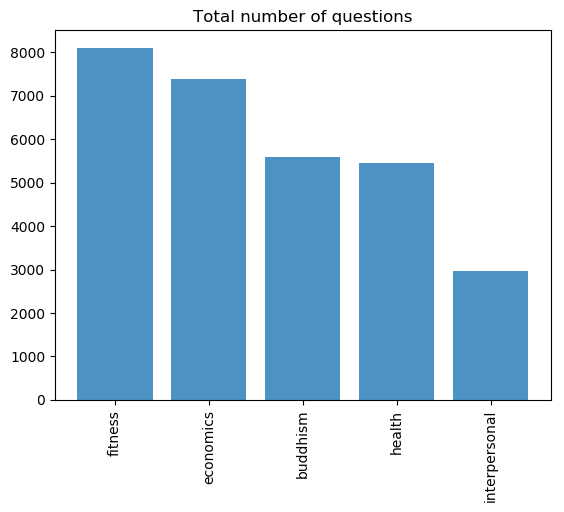
\includegraphics[width=0.32\linewidth]{../../01-python-code/00-workspace/01-graphs/post-counts-bar-graph} 
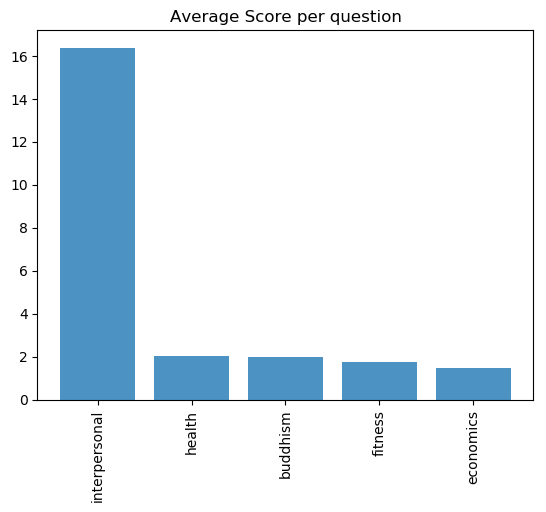
\includegraphics[width=0.32\linewidth]{../../01-python-code/00-workspace/01-graphs/ave-score-bar-graph} 
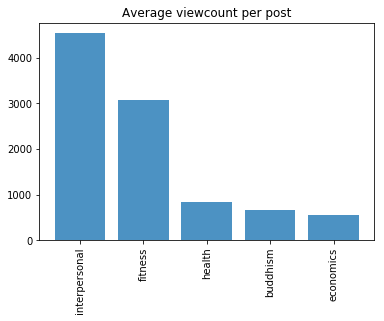
\includegraphics[width=0.32\linewidth]{../../01-python-code/00-workspace/01-graphs/ave-views-bar-graph} 
\\ \centering
{\footnotesize Source: Own calculations in PySpark.}
\end{minipage}
\end{figure}

\normalsize

Interpersonal has a substantially higher average \texttt{Score} per
question at over 16 compared to others which are just below, indicating
that this community hands out votes the easiest. However, Interpersonal
also has the highest \texttt{ViewCount}, signalling that it has the most
viewing activity from both community-members and non-community members
alike. When considering the composite variable,
\texttt{Score}/\texttt{ViewCount}, Interpersonal interestingly comes
last, showing that although they are overall the most generous at
handing out up-votes, when compensating for how much viewing traffic the
questions get the community actually has on average the least votes
being cast out of the amount of views questions get (due to many
non-community member views, many up-votes being offset by down-votes
i.e.~contentious issues??).

Needless to say, these communities appear to operate quite distinctly,
making predicting community engagement by a single topic-based-model
quite challenging, which would be contrary to the claim made by Ravi
\emph{et al.} (2014). The above average figures only display one
dimension however, so we further graph the density curves for all three
variables in figures blah through blah.

\subsection{A Clear Definition of the Response
Variable}\label{a-clear-definition-of-the-response-variable}

In order to robustly define a response variable capturing community
engagement, there are certain aspects of the data and functioning of the
StackExchange sites that should be discussed. First of all, although
questions on all StackExchange sites being open to the public, posting a
question in a community requires registration with an email address and
a username. Once registered, users start with a \emph{reputation} level
of 1
(\url{https://meta.stackexchange.com/questions/7237/how-does-reputation-work}).
The reputation levels key to my analysis are laid out as follows:

\setstretch{0.65}

\begin{itemize}
\item
  15: Users are allowed to ``up-vote'' questions and answers
\item
  125: Users can ``down-vote'' questions and answers
\item
  1000: Users can edit any question or answer.
\end{itemize}

\setstretch{1.25}

One factor is that there seems to be a less-than-full consensus of when
exactly to up- or
down-vote\footnote{https://meta.stackexchange.com/questions/12772/should-i-upvote-bad-questions}
despite general guidelines on StackExchange sites stating that up-votes
should be given if a question shows prior research, is clear and useful,
and down-voting the opposite.

One possible confounding factor for the response variable that is worth
considering is that questions can be edited, not only by the original
poster, but by anyone with a level of reputation of 1000 or more.
General cross-community guidelines for editing include addressing
grammar and spelling issues, clarifying concepts, correcting minor
mistakes, and adding related resources and links. The concern here is
that users could vote, comment and answer on substantially different
questions over time as a question is edited from it's original form.
\textbf{The simplifying assumption that I make here is that most edits,
if any at all, would happen quickly as moderators are made aware of
offending questions and thus the majority of views and votes would
happen on final, edited questions. I therefore choose final edited
question content to predict on.}

The contrasting reputation levels for up- and down-voting privileges (15
and 125 respectively) also lead to a \texttt{Score} variable that is
highly negatively skewed, making it more likely that questions will have
a higher \texttt{Score} and giving the appearance that most questions
are highly valued by a community. The density curves of the
\texttt{Score} variable per community in figure \ref{fig:density} below
confirm this. The negative skewness of all 5 curves is clearly evident,
and all except Interpersonal are steeply centred just after 0.

\footnotesize

\begin{figure}
\caption{\textbf{Density Plots}}
\label{fig:density}

\begin{center}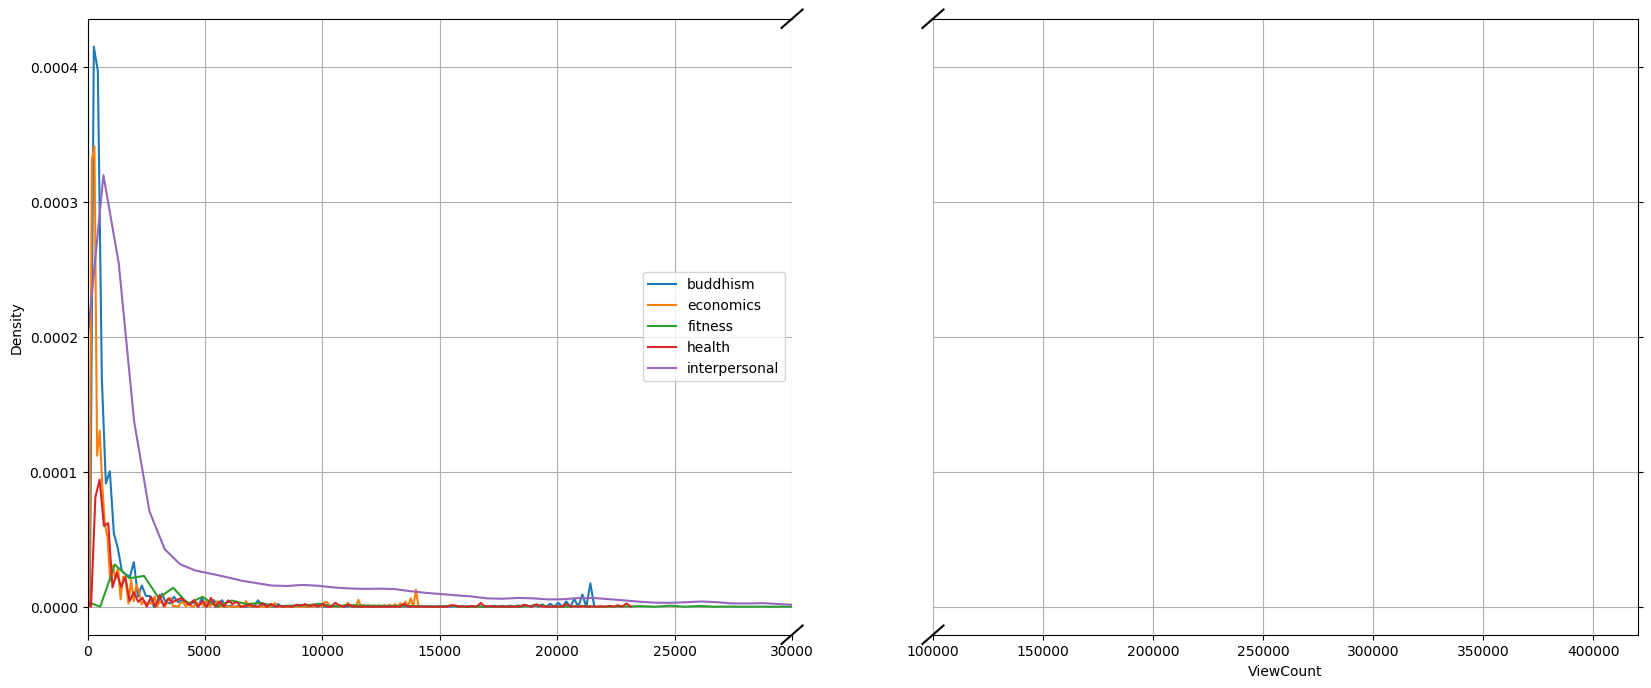
\includegraphics[width=0.8\linewidth]{../../01-python-code/00-workspace/01-graphs/views-density-plot} \end{center}



\begin{center}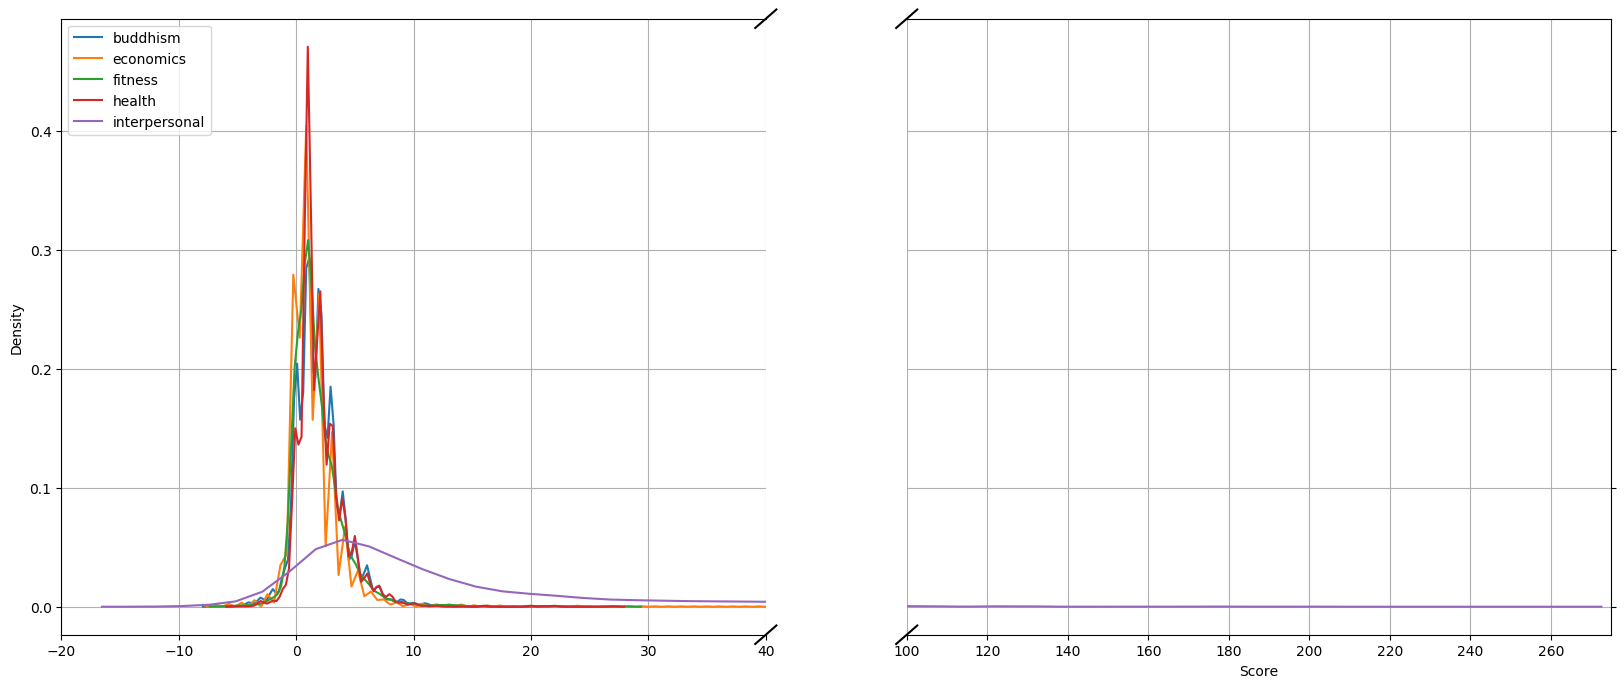
\includegraphics[width=0.8\linewidth]{../../01-python-code/00-workspace/01-graphs/score-density-plot} \end{center}
\centering {\footnotesize Source: Own calculations in PySpark.}
\end{figure}

\normalsize

Despite the negative skewness, because I am predicting a continuous
response variable as opposed to binary, \textbf{I believe this won't be
an issue.} It is just the way that the site functions and thus my
prediction model will not not be altered to try and force the data to my
whim.

A really interesting aspect of the data and of the functioning of the
StackExchange sites concerns the \texttt{Score} and \texttt{ViewCount}
variables. \textbf{As mentioned}, only members that have registered with
the community are able to up-vote and down-vote, thus contributing to
the \texttt{Score}, but owing to all questions being open to the public,
\texttt{ViewCount} variable registers views from 1) registered users
that can vote, 2) registered users that can't vote due to a reputation
level below 15), and 3) non-registered members.

This caveat influences the methodology of Ravi \emph{et al.} (2014) in
two ways. First, they decide to use a composite response variable,
\texttt{Score}/\texttt{ViewCount}, since thise would move in the
direction of taking the proportion of users that have decided to vote
out of the total number into account (i.e.~the percentage of voters that
decided to up-vote a question could be small in comparison to the total
amount of users that viewed the question). As they rightly point out,
considering \texttt{Score} alone might lead to conflating popularity
with their goal of measuring question quality, since a higher
\texttt{ViewCount} would definitely bias the \texttt{Score} variable
upwards owing to the unsymmetrical reputation privileges.

That said, here we have a look at the correlations between the
\texttt{Score} and \texttt{ViewCount} variable:

\footnotesize

\begin{longtable} {@{} cp{11cm} @{}}
\caption{\textbf{Best and Worst Fora Questions}}
\label{tab:bestworst}\\ 
\toprule
\textbf{Forum} & \textbf{Score/ViewCount Correlation} \\ 
\midrule
Buddhism & 0.441583990377997 \\
Economics & 0.29542738683698866 \\
Fitness & 0.35391344729176477 \\
Health & 0.14507264715830742 \\
Interpersonal & 0.8805605882358185 \\
\bottomrule
\end{longtable}\begin{center} Source: Own calculations in PySpark.\end{center}

\normalsize

I like to place this challenge in a framework of ``within-community''
engagement, and ``outer-community engagement''. Votes from community
members, and consequently the \texttt{Score} variable, is purely a
within-community metric since you have to be registered with the
community to contribute to this variable. \texttt{ViewCount} on the
other hand, is both a within- and outer- community engagement variable,
since it does not distinguish voting or non-voting status when
registering question views. I choose not to mix these two metrics and
focus solely on within-community engagement through the \texttt{Score}
variable - although this may mean popularity may be entangled in this
response variable I have chosen, I would assert that popularity is in
itself a measurement of community engagement and users would really only
be interested in this final \texttt{Score} prediction rather than
something like \texttt{Score}/\texttt{ViewCount}.

The second methodological adjustment that Ravi \emph{et al.} (2014) make
with their data is to only consider questions above a certain minimum
\texttt{ViewCount} threshold. Their reasoning behind this is so that
they can be more confident of the final dataset containing questions
that have been viewed by qualifying users that can vote, or in other
words their claim is that questions with higher \texttt{ViewCounts} have
a higher probability of having been seen by community members able to
vote.

I believe this is a false claim, since one could just as easily argue
that new questions that begin with a low \texttt{ViewCount} are more
likely to see engagement from proactive community members, especially if
these questions doesn't generate enough webpage activity to rise as the
top hit for search engines (which would lead to more non-community
member activity contribution to views). Since there is additionally no
data on the distribution of qualifying and non-qualifying user
contributions to the \texttt{ViewCount} variable, therefore I opt to not
disregard any questions below a certain \texttt{ViewCount} threshold.

Table \ref{tab:bestworst} displays the titles of a selection of
community questions with the highest and lowest \texttt{Scores}, i.e.~a
selection of the ``best'' and ``worst'' questions according to the
methodology I have chosen.

\footnotesize

\begin{longtable} {@{} cccp{11cm} @{}}
\caption{\textbf{Best and Worst Fora Questions}}
\label{tab:bestworst}\\ 
\toprule
\textbf{Forum} & \textbf{Score} & \textbf{ViewCount} & \textbf{Title} \\ 
\midrule
Buddhism &     55 &       6491 &  Is rebirth a delusional belief? \\
Buddhism &     -7 &        435 &       Why are buddhists hostile? \\
Buddhism &     -7 &        100 &        Who remembers the Buddha? \\
\hline
Economics &     94 &      17337 &  How will non-rich citizens make a living if jobs keep getting replaced by robots and are outsourced? \\
Economics &     -9 &        102 &                                      Has anyone made a successful economic prediction more than once? \\
\hline
Fitness &    111 &     132387 &  Is it healthy to exercise a muscle when it's still sore? \\
Fitness &     -7 &         51 &                       Gaining fat for muscles-stomach fat \\
\hline
Health &    103 &       5218 &                            How can I protect my eyesight when using computers? \\
Health &     -6 &        120 &  Would a stomach/bladder port allow for infinite and safe eating of junk food? \\
\hline
Interpersonal &    263 &      31487 &                     What to do if you are accidentally following someone? \\
Interpersonal &     -9 &       1327 &  How can I tell if family members consider my unvaccinated kids a threat? \\
Interpersonal &     -9 &        884 &             How to tell employees that I don't mean my insults seriously? \\
\bottomrule
\end{longtable}\begin{center} Source: Own calculations in PySpark.\end{center}

\normalsize

\textbf{Table \ref{tab:bestworst} appears to show that questions that
are considered the ``best'' tend to be honest and discussion-promoting,
whereas the ``worst'' questions are often sarcastic and probably not
genuinely looking for an answer - the questions from the Economics and
Fitness fora illustrate this. Social norms also appear to play a strong
part, since the ``worst'' question on the Interpersonal forum eludes to
children being unvaccinated, which I assume would upset many individuals
on the forum and lead to lowest \texttt{Score} per \texttt{ViewCount}
for that forum.} We can see that this is now validated.

I split that set of questions, \(Q\), into a training set
\(Q_\text{train}\) and testing set \(Q_\text{train}\) using a point in
time to mimic the reality of employing this tool at a certain point in
time with historical training data. With the chosen date of
\textbf{1/1/2017}, the ratio of \(Q_\text{train}\) to \(Q_\text{train}\)
are \ldots{}\ldots{}. for \ldots{}\ldots{}\ldots{} respectively.

\textbf{This addresses something that has not been considered in the
literature and introduces a temporal element into the analysis. While I
do not employ time-series models, I leave it to further research to
incorporate a way to ``remember'' which questions are good, so that in
future there are no duplicates.}

\subsection{\texorpdfstring{Model \label{Model}}{Model }}\label{model}

I employ a simple regularised regression with the \texttt{Body} and
\texttt{Title} as inputs from questions \(q_i\) out of
\(Q_\text{train}\), i.e.~the learning goal is to find a coefficient
vector \(\bm{\beta}\) that minimises the Root Mean Squared Error:

\begin{align} \label{rmse}
\underset{\bm{\beta}}{\text{minimise}} \quad \sqrt{ \frac{1}{|Q_\text{train}|} \sum_{ q_{i} \in Q_{\text{train}} } ( y_i - {\bm{\beta}\phi(\bm{x'}_i}) )^2 + \lambda \bm{\beta}\bm{\beta'} }
\end{align}

The \(y_i\) is the true value of the response variable,
\texttt{Score}/\texttt{ViewCount}, and \(\bm{\beta}\phi(\bm{x'}_i)\) is
the predicted response. \(\phi(\cdot)\) is a function on the features,
and leads to the feature engineering, of which lda is discussed in
section \ref{lda}. \(\lambda\) is the regularisation parameter
\ldots{}\ldots{}.

I use the \texttt{pyspark.sql.mllib} package in PySpark and inherent
online LDA learning framework to solve the optimisation problem
\ref{rmse}.

I use 2-fold cross validation - 2 because increasing the number of folds
did not lead to large gains in RMSE reduction, and also drastically
increased computation time.

\subsection{Feature Engineering}\label{feature-engineering}

A number of preprocessing steps was then applied to the question
\texttt{Body} and \texttt{Title} - HTML parsing for the question content
in the \texttt{Body} variable, tokenisation, removal of English
stopwords and Russian stopwords for Russian StackOverflow and stemming
of tokens.

\section{\texorpdfstring{Results
\label{Results}}{Results }}\label{results}

The results of the various models are displayed in tables. From it, we
can see this this and that.

\footnotesize

\begin{longtable}[htbp] {@{} lccc @{}} 
\caption{\textbf{Constant Mean Model}} 
\label{tab:mean_model} \\
\toprule
\textbf{Forum} &  \textbf{Train RMSE} &  \textbf{Test RMSE} &  \textbf{Time (s)} \\
\midrule
Buddhism      &              3.744804 &              3.026707 &                0.19 \\
Economics     &              3.558443 &              2.629807 &                0.20 \\
Fitness       &              5.630797 &              3.168150 &                0.37 \\
Health        &              4.331709 &              2.568920 &                0.29 \\
Interpersonal &             25.585999 &             16.252211 &                0.16 \\
\bottomrule
\end{longtable}\begin{center} Source: Own calculations in PySpark\end{center}

\normalsize

We use the mean of the training set as predictions for the test set in
table \ref{tab:mean_model}, which is the low benchmark. Interestingly,
test RMSE is lower for all communities than train RMSE, thus it appears
that there is substantially more noise in the training sets (remember
that the training sets are older questions as well).

This leads us to investigate the variation among train/test samples for
the communities:

\footnotesize

\begin{longtable}[htbp] {@{} lccc @{}} 
\caption{\textbf{Random 80/20 Train/Test Descriptives}} 
\label{tab:tr-te} \\
\toprule
\textbf{Forum} &  \textbf{Train StdDev} &  \textbf{Test StdDev} \\
\midrule
Buddhism & 3.68 & 3.33 \\
Economics & 3.51 & 2.96 \\
Fitness & 5.28 & 5.28 \\
Health & 4.22 & 3.54 \\
Interpersonal & 24.33 & 23.09 \\
\bottomrule
\end{longtable}\begin{center} Source: Own calculations in PySpark\end{center}

\normalsize

\footnotesize

\begin{longtable}[htbp] {@{} lccc @{}} 
\caption{\textbf{Temporal 80/20 Train/Test Descriptives}} 
\label{tab:tr-te} \\
\toprule
\textbf{Forum} &  \textbf{Train StdDev} &  \textbf{Test StdDev} \\
\midrule
Buddhism & 3.75 & 1.77 \\
Economics & 3.56 & 1.98 \\
Fitness & 5.63 & 2.2 \\
Health & 4.33 & 2.15 \\
Interpersonal & 25.59 & 11.72 \\
\bottomrule
\end{longtable}\begin{center} Source: Own calculations in PySpark\end{center}

\normalsize

Data has heterogeneity when considered temporally, possibly because of
interventions in communitites to effect answers?

\footnotesize

\begin{longtable}[htbp] {@{} lcccc @{}} 
\caption{\textbf{ViewCount Model}} 
\label{tab:vc_model} \\
\toprule
\textbf{Forum} &  \textbf{Train RMSE} &  \textbf{Test RMSE} &  \textbf{Test Gain (\%)} &  \textbf{Time (s)} \\
\midrule
Buddhism      &             3.374630 &          2.613928 &             13.638 &               5.22 \\
Economics     &             3.415546 &          2.394207 &              8.959 &               4.94 \\
Fitness       &             5.281202 &          2.798655 &             11.663 &               4.92 \\
Health        &             4.287559 &          2.522763 &              1.797 &               4.32 \\
Interpersonal &            12.321576 &          5.702388 &             64.913 &               4.30 \\
\bottomrule
\end{longtable}\begin{center} Source: Own calculations in PySpark\end{center}

\normalsize

Table \ref{tab:vc_model} is the high benchmark, since it is vacuous (the
final \texttt{ViewCount} of a question is not available for new
questions) and a higher \texttt{ViewCount} would definitely lead to
higher \texttt{Score}.

\footnotesize

\begin{longtable}[htbp] {@{} lcccccc @{}} 
\caption{\textbf{Tokens Model}} 
\label{tab:token_model} \\
\toprule
\textbf{Forum} &  \textbf{Train RMSE} &  \textbf{Test RMSE} &  \textbf{Test Gain (\%)} &  \textbf{Time (s)} & \textbf{Elastic Param} &  \textbf{Reg'tion Param} \\
\midrule
Buddhism      &          3.744804 &       3.026707 &           0.00 &           87.81 &               1.0 &               1.0 \\
Economics     &          3.558443 &       2.629807 &           0.00 &          139.93 &               1.0 &               1.0 \\
Fitness       &          5.630797 &       3.168150 &           0.00 &          141.84 &               1.0 &               1.0 \\
Health        &          4.331709 &       2.568920 &           0.00 &           91.37 &               1.0 &               1.0 \\
Interpersonal &         20.579032 &      17.264799 &           -6.23 &          120.35 &               1.0 &               1.0 \\
\bottomrule
\end{longtable}\begin{center} Source: Own calculations in PySpark\end{center}

\normalsize

The results of using unigram text of question titles and bodies is
displayed in table \ref{tab:token_model}. This model struggles
particularly, only predicting constant mean predictions for every
community except for Interpersonal, where it actually performs worse
than just predicting the mean by 6\%. Interestingly, the grid search
gives an elastic parameter of 1 and regularisation parameter of 1 for
all models.

DISCUSS WHY RMSE IS DIFFERENT PER COMMUNTIY

\section{\texorpdfstring{Limitations
\label{Limit}}{Limitations }}\label{limitations}

Different motivations behind voting.

Different interventions from StackExchange sites (nudges introduced
already.)

One aspect of this research that stands out as an area for further
research is the fact that only one target variable was considered (i.e.
\texttt{Score}/\texttt{ViewCount}) as a measurement of community
interaction, whereas in reality there are others already available in
the data. There are metrics recording how many interactions a question
receives, such as \texttt{AnswerCount} (the number of answers for a
question) and \texttt{CommentCount} (the number of comments for a
question), which all signify at least some engagement with a question,
although whether this is positive or negative engagement is unknown. In
response to this, one could construct a variable relating to the
linguistic sentiment of the answers (not comments, since comments need
not be directed at the original questioner), however the subtleties of
identifying sarcastic and condescending answers and comments might be
overly difficult, especially since communities would value pleasant
critical feedback.

Another variable that is a direct indication of questioner satisfaction
is whether they deem an answer to have successfully addressed their
question, which is recording in the variable \texttt{AcceptedAnswer}.
This variable is not without its own issues, since users may find
utility from multiple answers and neglect to formally select an accepted
answer at all, biasing the number of formally solved questions downwards
and confounding the response variable. Furthermore, answers are commonly
posted as comments and vice-versa (see
\url{https://meta.stackexchange.com/questions/17447/answer-or-comment-whats-the-etiquette}),
and this too would confound the predictive results for this variable.
Comments being posted as answers (i.e. ``clogging up'' the list of
answers), can be a case of users who don't have the required level of
reputation to comment yet or a case of users chasing reputation points
by using jokes, which obscurs the reputation measurement as users get
voted up for being humourous rather than their expertise. Treating this
variable as the target variable also situates the research problem in
terms of exclusive utility to the user, whereas the \texttt{Score}
variable is a more broader measurement of how the community values
questions, which in turn should translate into utility for the
questioner. One assumption that would mitigate issues surrounding the
\texttt{AcceptedAnswer} variable would state that the discussed
anomalies are not common enough and are not biased to specific posts
with an even and randomly distribution over the data it would not
significantly effect the results.

One last response variable for consideration is the number of times a
post is edited, the \texttt{EditCount}. This variable could have two
implications however - more edits signify more effort needed to bring
the question in the desired state (i.e.~it is inversely proportional to
positive community engagement), or more edits signify more energy
willingly devoted to improving the question because it will add value to
the community (and thus it is directly proportional to positive
community engagement).

Temporal aspect

\newpage

\section{\texorpdfstring{Recommendations for Further Research
\label{Recom}}{Recommendations for Further Research }}\label{recommendations-for-further-research}

\textbf{As has been discussed}, there are other response variables for
consideration, each with their own merits and disadvantages, however
further research could investigate these and address the issues
surrounding each response.

As mentioned, one limitation is that questions can be edited not only by
the original poster, but also by anyone with 2000 reputation or more.
One suggestion for further research would be investigating average
times-taken for events such as edits, answers, votes and views to
ascertain if the assumption of most votes occurring before edits is
permissable (NO DATA ON THIS THOUGH).

Another is that the above model does not take into account the temporal
nature of questions - i.e.~a good question that is asked will be
received positively by the community, however if a very similar question
is asked later on, the community will see that as ``lack of prior
research'' and will respond negatively. This analysis is but just a
first step in accurately predicting positive community reaction, so
further research could address the temporal model.

\newpage

\section{\texorpdfstring{Concluding Remarks
\label{Concl}}{Concluding Remarks }}\label{concluding-remarks}

The aim of this research was to predict the range of positive/negative
community engagement that questions elicit. I believe that no prior
research has endeavoured with the methodology here in this respective
framework to predict and capture community engagement. At the very
least, the research here has improved upon the extent of how community
engagement can be ascertained from online Q\&A communities, and has
yielded insight into how homogeneously community engagement exists over
diverse communities with various subject matter. I believe that using
this tool, online Q\&A users will be assisted in improving their
submitted questions which will enhance the productivity of all online
Q\&A communities wholly. Furthermore, room exists for implementation on
any assortment of Q\&A sites, counting Massive Open Online Courses.

\newpage

\section*{References}

\hypertarget{refs}{}
\hypertarget{ref-Agichtein2008}{}
Agichtein, E. \emph{et al.} (2008) `Finding high-quality content in
social media', in \emph{Proceedings of the 2008 international conference
on web search and data mining}. ACM, pp. 183--194. doi:
\href{https://doi.org/10.1145/1341531.1341557}{10.1145/1341531.1341557}.

\hypertarget{ref-Allamanis2013}{}
Allamanis, M. and Sutton, C. (2013) `Why, when, and what: Analyzing
stack overflow questions by topic, type, and code', in \emph{2013 10th
working conference on mining software repositories (msr)}. IEEE, pp.
53--56. doi:
\href{https://doi.org/10.1109/MSR.2013.6624004}{10.1109/MSR.2013.6624004}.

\hypertarget{ref-Anderson2012}{}
Anderson, A. \emph{et al.} (2012) `Discovering value from community
activity on focused question answering sites: a case study of stack
overflow', in \emph{Proceedings of the 18th acm sigkdd international
conference on knowledge discovery and data mining}. ACM, pp. 850--858.
Available at: \url{http://dl.acm.org/citation.cfm?id=2339665}.

\hypertarget{ref-Bian2009}{}
Bian, J. \emph{et al.} (2009) `Learning to recognize reliable users and
content in social media with coupled mutual reinforcement', in
\emph{Proceedings of the 18th international conference on world wide
web}. ACM, pp. 51--60. doi:
\href{https://doi.org/10.1145/1526709.1526717}{10.1145/1526709.1526717}.

\hypertarget{ref-Blei2003}{}
Blei, D. M., Ng, A. Y. and Jordan, M. I. (2003) `Latent Dirichlet
Allocation', \emph{Journal of Machine Learning Research}, 3, pp.
993--1022.

\hypertarget{ref-Chiang2010}{}
Chiang, D. \emph{et al.} (2010) `Bayesian Inference for Finite-State
Transducers', in \emph{Human language technologies: The 2010 annual
conference of the north american chapter of the association for
computational linguistics}. Association for Computational Linguistics
(June), pp. 447--455. Available at:
\href{http://www.isi.edu/\%7B~\%7Dsravi/pubs/naacl2010\%7B/_\%7Dbayes-fst.pdf}{http://www.isi.edu/\{\textasciitilde{}\}sravi/pubs/naacl2010\{\textbackslash{}\_\}bayes-fst.pdf}.

\hypertarget{ref-Fligner1986}{}
Fligner, M. and Verducci, J. S. (1986) `Distance based ranking models',
\emph{Journal of the Royal Statistical Society: Series B
(Methodological)}, 48(3), pp. 359--369.

\hypertarget{ref-Jeon2006}{}
Jeon, J. \emph{et al.} (2006) `A framework to predict the quality of
answers with non-textual features', in \emph{Proceedings of the 29th
annual international acm sigir conference on research and development in
information retrieval}. ACM, pp. 228--235. doi:
\href{https://doi.org/10.1145/1148170.1148212}{10.1145/1148170.1148212}.

\hypertarget{ref-Li2010}{}
Li, B. and King, I. (2010) `Routing questions to appropriate answerers
in community question answering services', in \emph{Proceedings of the
19th acm international conference on information and knowledge
management}. ACM, pp. 1585--1588. doi:
\href{https://doi.org/10.1145/1871437.1871678}{10.1145/1871437.1871678}.

\hypertarget{ref-Li2012}{}
Li, B. \emph{et al.} (2012) `Analyzing and predicting question quality
in community question answering services', in \emph{Proceedings of the
21st international conference on world wide web}. ACM, pp. 775--782.
doi:
\href{https://doi.org/10.1145/2187980.2188200}{10.1145/2187980.2188200}.

\hypertarget{ref-Li2011}{}
Li, B., King, I. and Lyu, M. R. (2011) `Question routing in community
question answering', in \emph{Proceedings of the 20th acm international
conference on information and knowledge management}. ACM, pp.
2041--2044. doi:
\href{https://doi.org/10.1145/2063576.2063885}{10.1145/2063576.2063885}.

\hypertarget{ref-Liu2008}{}
Liu, Y., Bian, J. and Agichtein, E. (2008) `Predicting information
seeker satisfaction in community question answering', in
\emph{Proceedings of the 31st annual international acm sigir conference
on research and development in information retrieval}. ACM (Section 2),
pp. 483--490. doi:
\href{https://doi.org/10.1145/1390334.1390417}{10.1145/1390334.1390417}.

\hypertarget{ref-Qu2009}{}
Qu, M. \emph{et al.} (2009) `Probabilistic question recommendation for
question answering communities', in \emph{Proceedings of the 18th
international conference on world wide web}. ACM (2), pp. 1229--1230.
doi:
\href{https://doi.org/10.1145/1526709.1526942}{10.1145/1526709.1526942}.

\hypertarget{ref-Ravi2014}{}
Ravi, S. \emph{et al.} (2014) `Great Question! Question Quality in
Community Q\&A.', in \emph{Eighth international aaai conference on
weblogs and social media}. (1), pp. 426--435.

\hypertarget{ref-Riahi2012}{}
Riahi, F. \emph{et al.} (2012) `Finding expert users in community
question answering', in \emph{Proceedings of the 21st international
conference on world wide web}. ACM, pp. 791--798. doi:
\href{https://doi.org/10.1145/2187980.2188202}{10.1145/2187980.2188202}.

\hypertarget{ref-Shah2010}{}
Shah, C. and Pomerantz, J. (2010) `Evaluating and predicting answer
quality in community QA', in \emph{Proceedings of the 33rd international
acm sigir conference on research and development in information
retrieval}. ACM (March 2008), pp. 411--418. doi:
\href{https://doi.org/10.1145/1835449.1835518}{10.1145/1835449.1835518}.

\hypertarget{ref-Shah2018}{}
Shah, V. \emph{et al.} (2018) `Adaptive matching for expert systems with
uncertain task types', in \emph{2017 55th annual allerton conference on
communication, control, and computing (allerton)}. IEEE, pp. 753--760.
doi:
\href{https://doi.org/10.1109/ALLERTON.2017.8262814}{10.1109/ALLERTON.2017.8262814}.

\hypertarget{ref-Sung2013}{}
Sung, J., Lee, J.-g. and Lee, U. (2013) `Booming Up the Long Tails:
Discovering Potentially Contributive Users in Community-Based Question
Answering Services', in \emph{Seventh international aaai conference on
weblogs and social media}, pp. 602--610.

\hypertarget{ref-Szpektor2013}{}
Szpektor, I., Maarek, Y. and Pelleg, D. (2013) `When relevance is not
enough: promoting diversity and freshness in personalized question
recommendation', in \emph{Proceedings of the 22nd international
conference on world wide web}. ACM, pp. 1249--1260.

\hypertarget{ref-Tian2013}{}
Tian, Q., Zhang, P. and Li, B. (2013) `Towards Predicting the Best
Answers in Community-Based Question-Answering Services', in
\emph{Seventh international aaai conference on weblogs and social
media}, pp. 725--728.

\hypertarget{ref-Wu2008}{}
Wu, H., Wang, Y. and Cheng, X. (2008) `Incremental probabilistic latent
semantic analysis for automatic question recommendation', in
\emph{Proceedings of the 2008 acm conference on recommender systems}.
ACM, p. 99. doi:
\href{https://doi.org/10.1145/1454008.1454026}{10.1145/1454008.1454026}.

\hypertarget{ref-Zhou2012}{}
Zhou, T. C., Lyu, M. R. and King, I. (2012) `A classification-based
approach to question routing in community question answering', in
\emph{Proceedings of the 21st international conference on world wide
web}. ACM, pp. 783--790. Available at:
\url{http://www2012.wwwconference.org/proceedings/companion/p783.pdf}.

% code for wordcount (INCOMPLETE)
\newcommand\wordcount{
    \immediate\write18{texcount -sub=section \jobname.tex  | grep "Section" |     sed -e 's/+.*//' | sed -n \thesection p > 'count.txt'}
(\input{count.txt}words)}

\end{document}
